% Context and motivation
Natural language processing methods for the generation of symbolic music have experienced significant advancements in recent years.
The transformer architecture, introduced by Vaswani et al. in 2017, has been used to generate scores for various instruments, in diverse styles and genres\cite{vaswani_attention_2023, le_natural_2024}.
An unpublished user study conducted by Bacot et al. showed a potential need for accompaniment generation tools for guitarists.
The questionnaire was answered by 31 guitarist-composers, and 7 of them followed up with an interview.
During the interviews, several guitarists answered that they would like to be able to generate bass guitar lines and drum parts without requiring familiarity with the instruments.
Indeed, guitarists often resort to writing basic bass lines to accompany their compositions, and an AI tool could perform this functional task for them\cite{bacot_tablature_2025}.

% Objectives
This need is the starting point for this project, proposed by the Algomus team, part of the CRIStAL laboratory.
We focus on the conditional aspect of symbolic music generation, for an instrument that has not been thoroughly studied yet: the bass guitar.
Specifically, the goal is to generate bass guitar tablatures given other instruments' scores, in the context of western popular music.
Our objective is to try several combinations of conditioning instruments and to evaluate the quality of the generated tablatures both numerically and with the help of musicians.


% Terms definition (tablature, add the period when it was used)
% Difference between guitar and bass (role in the music)
To better understand what is at stake in this challenge, we will begin by precisely defining the role of the bass guitar in the context of western popular music.
Since the human ear perceives low-frequency pulses more distinctly, the bass guitar is considered part of the rhythmic section of the band (together with the drums)\cite{hove_superior_2014}.
However, the bass guitar also performs a harmonic — and sometimes melodic — role in the music, sustaining the lead instruments and adding depth to the composition.
Its adaptability makes the bass guitar a crucial component across various genres of western popular music.


Historically, tablatures have been used since the Renaissance period as a simplified notation system for string instruments like the lute.
Originating around the 16th century, tablatures were an intuitive alternative to staff notation, allowing musicians to bypass the complexity of interpreting pitches.
This system explicitly linked symbols to physical actions on the instrument, such as pressing specific frets or strings.
As a result, tablatures gained popularity among amateur and professional musicians alike.
In modern times, tools like GuitarPro have digitalized tablatures, further extending their use for learning, practice, and composition in genres ranging from classical to popular music\cite{sarmento_dadagp_2021}.

% add a fig Time is running out, melodic and rhythmic bass
\begin{figure}[h!]
    \centering
    \begin{minipage}{0.45\textwidth}
        \centering
        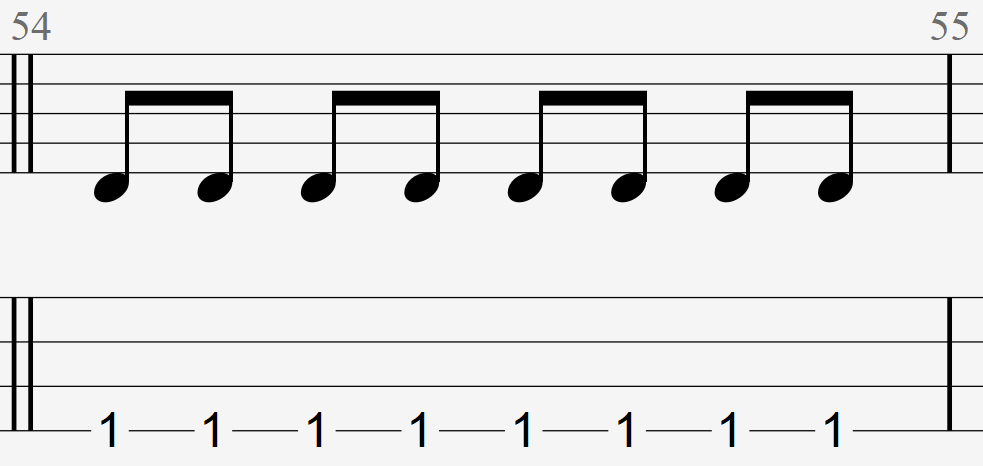
\includegraphics[width=.5\linewidth]{../images-figures/rhythmic_tab_TIRO.png}
    \end{minipage}%
    \hfill
    \begin{minipage}{0.45\textwidth}
        \centering
        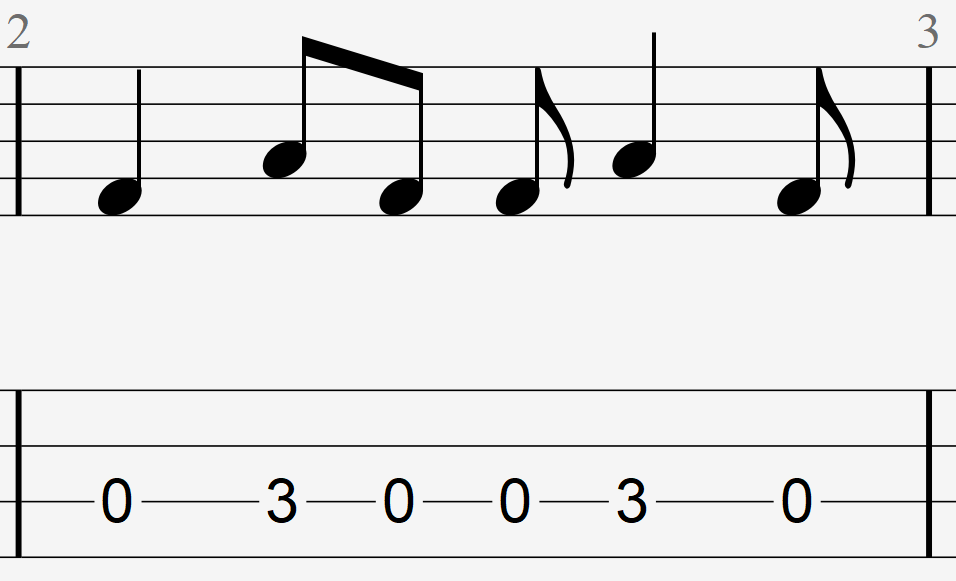
\includegraphics[width=.5\linewidth]{../images-figures/melodic_tab_TIRO.png}
    \end{minipage}
    \caption{Rhythmic (left) and melodic (right) extracts in Time is Running Out by Muse}
    \label{fig:bass_tab_TIRO}
\end{figure}


Figure~\ref{fig:bass_tab_TIRO} shows a tablature and score extract of both a rhythmic and a more melodic bass.
Scores display the notes to play, while tablatures show the fingering to use on the instrument.
More precisely, each line of the tablature represents a string of the instrument, and the numbers indicate the fret to press on the string.
For instance, in the figure on the right, the bassist will start by playing the fourth string with the first fret pressed.
Tablatures do not contain rhythmic information, which is why they are generally combined with scores.
Otherwise, the musician must know the song to play it correctly.


% Abstract challenges: (high-level such as: propose an informatic representation of music...)
Generating bass guitar tablatures presents several challenges.
At a high level, we first need to scrap and preprocess large datasets of music scores.
Then, we need to design a computational representation of music that is adapted to the task of generating bass guitar tablatures.
That is, a way to encode music scores in a meaningful way for the transformer architecture we will use.
Concerning the generation, we will start by leveraging state-of-the-art models but will adapt and tune them to the task at hand.